\section{Ασφαλής Υπολογισμός Συνάρτησης - Μη-Συνειδητή Μεταφορά}
\label{sec:OT}
\index{Ασφαλής}
Στην ενότητα αυτή θα ασχοληθούμε με ένα βασικό κρυπτογραφικό πρόβλημα τον \emph{Ασφαλή Υπολογισμό Συνάρτησης} \gls{SFE} και έναν τρόπο υλοποίησης του, τη \emph{Μη-Συνειδητή Μεταφορά} (η οποία είναι γνωστή κυρίως με τον αντίστοιχο αγγλικό όρο \gls{OT}). 

\begin{definition}{Ασφαλής Υπολογισμός Συνάρτησης}
$m$ οντότητες θέλουν να υπολογίσουν από κοινού τη συνάρτηση $f(x_1,x_2,\cdots,x_n)$. Κάθε οντότητα $m_i$ συνεισφέρει στον υπολογισμό τη δική της είσοδο $x_i$. Ο υπολογισμός πρέπει να θεωρείται ασφαλής δηλαδή να μην διαρρέει καμία επιπλέον πληροφορία εκτός από το αποτέλεσμα. 
\end{definition}

Στον παραπάνω ορισμό πρέπει να λάβουμε υπόψιν μας επιπλέον περιορισμούς, όπως για παράδειγμα την υπολογιστική πολυπλοκότητα, το πλήθος των bits που είναι απαραίτητο για την επικοινωνία και τον συγχρονισμό των οντοτήτων ώστε να εκτελέσουν τον υπολογισμό της συνάρτησης. Σε μία γενίκευση του παραπάνω προβλήματος κάθε οντότητα πρέπει να υπολογίσει τη δική της συνάρτηση, ζητώντας είσοδο από τις υπόλοιπες. Γενικά είναι αποδεκτός οποιοσδήποτε υπολογισμός με οποιεσδήποτε ανταλλαγές μηνυμάτων, οπότε προκύπτει μία ευρύτερη περιοχή, ο \emph{Ασφαλής υπολογισμός Πολλών-Μερών} (\gls{MPC}), με την οποία θα ασχοληθούμε σε επόμενη ενότητα. 

Αξίζει να τονίσουμε πως οι παραπάνω υπολογισμοί, όπως και πολλά άλλα στη σύγχρονη κρυπτογραφία, θα μπορούσαν να υλοποιηθούν με χρήση μιας έμπιστης τρίτης οντότητας. Φυσικά κάτι τέτοιο δεν είναι αποδεκτό καθώς η εμπιστοσύνη πρέπει να παρέχεται από το κρυπτογραφικό πρωτόκολλο που ακολουθείται. 

\subsection{Το πρόβλημα των εκατομμυριούχων}

Ένα γλαφυρό παράδειγμα της αναγκαιότητας για ασφαλή υπολογισμό συνάρτησης τέθηκε από τον Andrew Yao \cite{yao_protocols_1982} το 1982 ως εξής: 

Οι εκατομμυριούχοι (από την συνεχή χρήση του ονόματός τους) Alice και Bob, θέλουν να μάθουν ποιος από τους δύο είναι πλουσιότερος, χωρίς όμως να αποκαλύψουν ακριβώς την έκταση της περιουσίας τους. Το πρόβλημα αυτό αντιστοιχεί στον υπολογισμό της συνάρτησης δύο εισόδων ($m=2$):
\begin{center}
$f(x_a,x_b) = a$ if $x_a > x_b$ else $b$
\end{center}
Στη διατύπωση του προβλήματος είναι δημόσια γνωστό το εύρος που κυμαίνονται οι περιουσίες από $1$ έως κάποια τιμή $n$. Αν εκμεταλλευτούμε το γεγονός αυτό τότε μπορεί να προκύψει μία λύση, η οποία περιγράφηκε αρχικά και από τον ίδιο τον Yao στο \cite{yao_protocols_1982}.

\begin{itemize}
\item Ο Bob δημιουργεί $n$ ταυτόσημα κουτιά. 
\item Επιλέγει έναν αριθμό, τον οποίο τοποθετεί στο κουτί $b$.
\item Τα υπόλοιπα κουτιά τα γεμίζει με ένα τυχαίο αριθμό, ο οποίος δεν έχει κάποια ιδιαίτερη σημασία και θεωρείται αναλώσιμος.
\item Όλα τα κουτιά αποστέλλονται στην Alice.
\item H Alice με τη σειρά της τα ανοίγει. 
\item Αφήνει το περιεχόμενο στα πρώτα $a$ από αυτά αμετάβλητο, ενώ αυξάνει κατά 1 τα υπόλοιπα $n-a$.
\item Όλα τα κουτιά αποστέλλονται στον Bob.
\item Αν ο αριθμός του Bob (αυτός που βρίσκεται στο κουτί $b$) έχει αλλάξει, τότε αυτός είναι πλουσιότερος, ενώ αν έχει παραμείνει ο ίδιος τότε η Alice είναι πλουσιότερη.
\end{itemize}

Παρατηρούμε ότι το παραπάνω πρωτόκολλο, αν και λύνει το πρόβλημα, έχει κάποια προβλήματα. Για παράδειγμα o Bob μπορεί να μάθει την περιουσία της Alice, αν κρατήσει αρχείο των αριθμών που έχει τοποθετήσει σε κάθε κουτί. Επιπλέον με την παραπάνω περιγραφή μόνο ο Bob μαθαίνει ποιος είναι πλουσιότερος. Για να μάθει και η Alice πρέπει το πρωτόκολλο να εκτελεστεί με αντιστροφή των ρόλων. Σε αυτή την περίπτωση ο Bob μπορεί να κλέψει αλλάζοντας την τιμή του $b$ και θέτοντας την ίση με το $n$, έτσι ώστε να φαίνεται πάντα πλουσιότερος από την Alice. 

\subsection{Ανταλλαγή Μυστικών}
Ο Rabin στο \cite{rabin_eos} προσπάθησε να επιλύσει κάποια από τα παραπάνω προβλήματα βάζοντας αυστηρότερες προϋποθέσεις στο πρωτόκολλο. Συγκεκριμένα, γενίκευσε το πρόβλημα βάζοντας την Alice και τον Bob να ανταλλάξουν τα μυστικά τους $s_a, s_b$, με τους εξής κανόνες:
\begin{itemize}
\item Δεν μπορεί να χρησιμοποιηθεί έμπιστη τρίτη οντότητα
\item Κανένας δεν πρέπει να μπορεί να κλέψει ή να τερματίσει το πρωτόκολλο, αφού μάθει το μυστικό του άλλου
\item H ανταλλαγή πρέπει να είναι ταυτόχρονη
\end{itemize}

Η πρώτη παρατήρηση σε ένα τέτοιο σύστημα είναι ότι οποιοδήποτε τετριμμένο πρωτόκολλο για το πρόβλημα αυτό είναι προβληματικό: 
Έστω ότι τα μυστικά μπορούν να υπολογιστούν από την ανταλλαγή:
\begin{itemize}
\item $s_a = f(a_1,a_2, \cdots , a_n)$
\item $s_b = g(b_1,b_2, \cdots, b_n)$
\end{itemize}
Πάντοτε υπάρχει κάποιο $k$ ώστε το $s_a$ να μπορεί να υπολογιστεί από τα $a_1,a_2, \cdots , a_k$ αλλά το $s_b$ να μην μπορεί να υπολογιστεί από $b_1,b_2, \cdots, b_{k-1}$. Με απλά λόγια, το πρωτόκολλο μπορεί να τερματιστεί νωρίτερα από έναν από τους δύο συμμετέχοντες, μόλις αυτός πάρει αυτό που θέλει.

Για να επιλύσει το πρόβλημα αυτό ο Rabin χρησιμοποίησε την έννοια της Μη-Συνειδητής Μεταφοράς. Σε αυτήν, με πολύ απλά λόγια, ο αποστολέας ενός μηνύματος \emph{δεν μπορεί να μάθει αν ο παραλήπτης το έλαβε}. Για την υλοποίηση τής χρησιμοποιήθηκε το πρόβλημα των τετραγωνικών υπολοίπων \ref{sec:quadres}. Συγκεκριμένα ο αποστολέας θέλει  να στείλει την παραγοντοποίηση ενός αριθμού στον παραλήπτη ο οποίος θα την λάβει με πιθανότητα ${1}/{2}$.

\begin{itemize}
\item Η Alice και ο Bob διαθέτουν τα κλειδιά $k_a, k_b$ για κάποιο σχήμα δέσμευσης.
\item H Alice διαλέγει έναν \gls{RSA} modulus $n_a = p_a \dot q_a$ τον οποίο και στέλνει στον Bob χωρίς φυσικά να αποκαλύψει τους πρώτους παράγοντες.
\item O Bob διαλέγει κάποιο $x \leq n_a$ και υπολογίζει το $c = x^2 \pmod  n_a$. 
\item Στη συνέχεια αποστέλλει το $c$ και μία δέσμευση στο x $E_{k_b}(x)$.
\item Η Alice εφόσον διαθέτει την παραγοντοποίηση του $n_a$ μπορεί να υπολογίζει μία τετραγωνική ρίζα του $c$ χρησιμοποιώντας το κινέζικο θεώρημα των υπολοίπων (βλ. \ref{sec:CRT}).
\item Η ρίζα αυτή $x_1$ αποστέλλεται στον Bob.
\item Στην συνέχεια ο Bob ελέγχει αν το $x_1=x \pmod n_a$ ή αν $x_1= - x \pmod n_a$. Σε αυτή την περίπτωση δεν μπορεί να μάθει την παραγοντοποίηση του $n_a$. Στην αντίθετη περίπτωση όμως κάτι τέτοιο είναι δυνατό χρησιμοποιώντας τον αλγόριθμο του Ευκλείδη.
\end{itemize}

Χρησιμοποιώντας το παραπάνω πρωτόκολλο ως συστατικό, η ανταλλαγή μυστικών μπορεί να επιτευχθεί ως εξής:
\begin{itemize}
\item Η Alice χρησιμοποιεί μη συνειδητή μεταφορά για την παραγοντοποίηση ενός αριθμού $n_a$
\item Ο Bob χρησιμοποιεί μη συνειδητή μεταφορά για την παραγοντοποίηση ενός αριθμού $n_b$
\item Και οι δύο συμμετέχοντες θέτουν μια τιμή $v_a = 0$ και $v_b = 0$ αν και μόνο ν έλαβαν την παραγοντοποίηση των $n_b, n_a$ αντίστοιχα.
\item Υπολογίζουν αντίστοιχα τις τιμές $e_a = v_a \xor s_a$ και $e_b = v_b \xor s_b$ τις οποίες και ανταλλάσσουν.
\item Στη συνέχεια ενσωματώνουν τα μυστικά $s_a,s_b$ σε μηνύματα $m_a, m_b$ τα οποία και κρυπτογραφούν χρησιμοποιώντας το \gls{RSA} με κλειδιά τα $n_a, n_b$.
\item Αν $v_a = 0$ τότε η Alice μπορεί να αποκρυπτογραφήσει το $m_b$ και κατά συνέπεια $e_a = s_a$ οπότε ο Bob έχει λάβει το μυστικό. Αντίστοιχα και για τον Bob. 
\end{itemize}

\subsection{Μη-Συνειδητή Μεταφορά (Oblivious Transfer)}

Οι Even, Goldreich, Lempel στο \cite{even_randomized_1985} έδωσαν έναν αυστηρό ορισμό της Μη-Συνειδητής Μεταφοράς έχοντας ως πρότυπο την έννοια της μετάδοσης με θόρυβο.

\begin{figure}
	\centering
		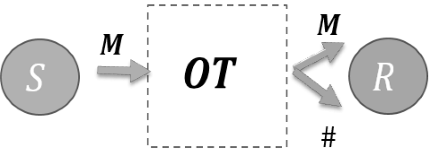
\includegraphics[width=0.8\textwidth]{Ch9/ot.png}
	\caption{Μη-Συνειδητή Μεταφορά}
	\label{fig:OT}
\end{figure}

\begin{definition}
Ένα πρωτόκολλο Μη-Συνειδητής Μεταφοράς $OT(S,R,M)$ είναι ένα πρωτόκολλο με το οποίο ένας αποστολέας $S$ μεταφέρει σε έναν παραλήπτη $R$ το μήνυμα $M$ έτσι ώστε:
\begin{itemize}
\item o $R$ λαμβάνει το $M$ με πιθανότητα $\frac{1}{2}$. Αν δεν λάβει το μήνυμα δεν μαθαίνει καμία επιπλέον πληροφορία.
\item Η εκ των υστέρων (\textsl{a posteriori}) πιθανότητα για τον $S$ για το συμβάν ο $R$ να λάβει το $M$ είναι $\frac{1}{2}$.
\item Οποιαδήποτε απόπειρα παράκαμψης του πρωτοκόλλου είναι άμεσα ανιχνεύσιμη.
\end{itemize}
\end{definition}

Επιπλέον όρισαν μία παραλλαγή την $1$-από-$2$ Μη-Συνειδητή Μεταφορά $OT_1^2(S,R,$ $M_1,M_2)$ ως το πρωτόκολλο στο οποίο ο $R$ επιλέγει μεταξύ δύο μηνυμάτων για μεταφορά με πιθανότητα ${1}/{2}$ και ο $S$ το μεταφέρει χωρίς ασφαλώς  να γνωρίζει ποιο μετέφερε. Μπορούμε να προσομοιώσουμε την τυχαία επιλογή χρησιμοποιώντας ένα bit.

\begin{figure}
	\centering
		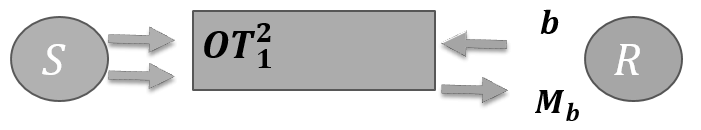
\includegraphics[width=0.8\textwidth]{Ch9/ot12.png}
	\caption{$1$-από-$2$ Μη-Συνειδητή Μεταφορά}
	\label{fig:OT12}
\end{figure}

Μια γενικευμένη παραλλαγή μπορεί να οριστεί ως $1$-από-$n$ Μη-Συνειδητή Μεταφορά $OT_1^n(S,R,M_1,\cdots,M_n)$ όπου ο $R$ επιλέγει μεταξύ $n$ μηνυμάτων να λάβει το $i$. Φυσικά ο $S$ δεν το μαθαίνει, ενώ ο $R$ δεν μαθαίνει τα $M_j, j \neq i$.

Επίσης μπορεί να οριστεί η $k$-από-$n$ Μη-Συνειδητή Μεταφορά με δύο παραλλαγές. Στην πρώτη από αυτές ο $R$ λαμβάνει ταυτόχρονα $k$ μηνύματα, ενώ στη δεύτερη η μεταφορά γίνεται σειριακά, με δυνατότητα τροποποίησης επιλογών με βάση τις ήδη ληφθείσες (adaptive $k$-από-$n$). 

\begin{theorem} 
$OT_1^2 \Leftrightarrow OT$
\end{theorem}

\begin{proof}
Οι Even, Goldreich, Lempel στο \cite{even_randomized_1985} απέδειξαν ότι $OT_1^2 \Rightarrow OT$ ενώ αργότερα ο Crepeau \cite{crepeau_equivalence_1988} απέδειξε ότι $OT  \Rightarrow OT_1^2$.

\begin{lemma}
$OT_1^2 \Rightarrow OT$
\end{lemma}
\begin{proof}

Ο $S$ θέλει να αποστείλει ένα μήνυμα $M$ με πιθανότητα $\frac{1}{2}$ στον $R$. Θέτει ως είσοδο το $M$ στην μηχανή $OT$ η οποία δημιουργεί ένα επιπλέον μήνυμα $M'$ (τυχαίο) για να το χρησιμοποιήσει εσωτερικά στην δεδομένη $OT_1^2$ μηχανή, η οποία έχει δύο εισόδους όπως φαίνεται άλλωστε και από το παρακάτω σχήμα.

\begin{figure}
	\centering
		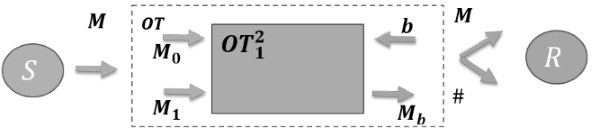
\includegraphics[width=0.8\textwidth]{Ch9/ot_from_ot12.png}
	\caption{$OT$ από $OT_1^2$}
	\label{fig:OTfromOT12}
\end{figure}

Επιπλέον δημιουργεί δύο τυχαία bits ακόμα, το $b$ για προσομοίωση του άλλου άκρου και το $b'$ για την ρύθμιση της εισόδου στην $OT_1^2$. Συγκεκριμένα: Αν $b'=0$ τότε εισάγει στην $OT_1^2$ το ζεύγος $(M_0,M_1)=(M,M')$ ενώ αν $b'=1$ εισάγει το ζεύγος $(M_0,M_1)=(M',M)$. 

Σε κάθε περίπτωση η $OT$ εξάγει στον παραλήπτη το $M_b$ που έχει εξάγει η $OT_1^2$. Έτσι $b=b'$ τότε θα εξαχθεί το $M$ ενώ σε διαφορετική περίπτωση το $M'$ που θα εκληφθεί ως θόρυβος. 

Έτσι ο $R$ μαθαίνει το $M$ με πιθανότητα ${1}/{2}$ και προσομοιώνεται πλήρως η μηχανή $OT$.

\end{proof}
\begin{lemma}
$OT \Rightarrow OT_1^2$
\end{lemma}

\begin{proof}
Για την αντίστροφη κατεύθυνση, δηλαδή για τη δημιουργία μιας μηχανής $OT_1^2$ χρησιμοποιώντας $OT$, ο Crepeau \cite{crepeau_equivalence_1988} αρχικά όρισε μία μηχανή $OT_p$ η οποία μεταφέρει κάποιο μήνυμα με πιθανότητα $p$. Είναι φανερό ότι η μηχανή αυτή αποτελεί γενίκευση της μηχανής $OT$.

\begin{figure}
	\centering
		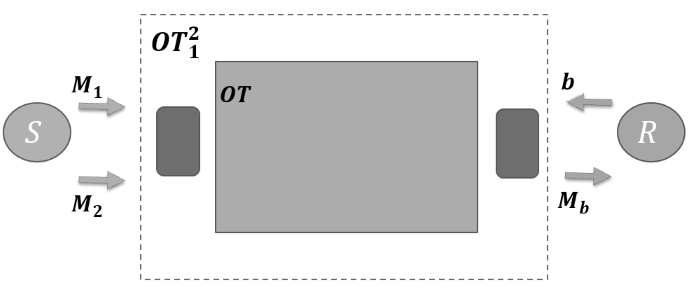
\includegraphics[width=0.8\textwidth]{Ch9/ot12_from_ot.png}
	\caption{$OT_1^2$ από $OT$}
	\label{fig:OT12fromOT}
\end{figure}

Στη συνέχεια απέδειξε ότι $OT_p \Rightarrow OT_1^2$. Ο $S$ στέλνει κανονικά τα μηνύματα $M_0, M_1$ και ο $R$ εισάγει το bit $b$.
Εσωτερικά λοιπόν κατασκευάζεται ένα διάνυσμα από bit $\vec{s}$, τα οποία στέλνονται \emph{διαδοχικά} στη μηχανή $OT_p$. 

Ανάλογα με το $b$ σε κάποιες από τις θέσεις του $\vec{s}$ η μεταφορά θα επιτύχει (στο σύνολο δεικτών $I_b$) ενώ σε κάποιες θα αποτύχει (στο σύνολο δεικτών $I_{1-b}$). Με βάση την πιθανοτική ανάλυση της $OT_p$ με πολύ μεγάλη πιθανότητα, το σύνολο $I_b$ μπορεί να βρεθεί, ενώ το σύνολο $I_{1-b}$ θα περιέχει τουλάχιστον μία τιμή όπου απέτυχε η μεταφορά $OT$.

Τελικά αποστέλλεται στη μηχανή $OT$ το $M_{\xor_{i \in I_b}} s_i, \b \in \{0,1\}$. H μία από τις παραπάνω XOR θα αποτύχει και έτσι ακριβώς ένα από τα $M_0, M_1$ θα μεταφερθεί. Δηλαδή έχουμε $OT_1^2$.
\end{proof}

\end{proof}

\subsection{Πρακτική κατασκευή}
Σε πρακτικό επίπεδο, για να κατασκευάσουμε ένα σύστημα $OT_1^2$ μπορούμε να χρησιμοποιήσουμε ένα κρυπτοσύστημα δημοσίου κλειδιού που έχει την ιδιότητα $\MSG = \CPH$. Για να υλοποιηθεί η μη συνειδητή μεταφορά των $M_0, M_1$ ο $R$ επιλέγει τυχαία δύο συμβολοσειρές $x_0, x_1$.
Τώρα για να πάρει το $M_0$ προχωρά στα εξής βήματα:
\begin{itemize}
\item Στέλνει στον $S$ το $(Enc(x_0),x_1)$
\item Ο $R$ αποκρυπτογραφεί, παράγοντας το $(x_0, Dec(x_1))$. Η αποκρυπτογράφηση μπορεί να γίνει και στις δύο περιπτώσεις λόγω της ιδιότητας του κρυπτοσυστήματος, αλλά φυσικά μόνο στην περίπτωση του $x_0$ έχει νόημα.
\item Τελικά ο $S$ αποστέλλει το $(M_0 \xor x_0, M_1 \xor Dec(x_1))$
\item Τελικά ο $R$ ανακτά το $M_0$ με XOR του πρώτου συστατικού: $M_0 \xor x_0 \xor x_0$
\end{itemize}
 
\subsection{Ασφαλής υπολογισμός συνάρτησης}
\label{sec:YAOSFE}
\index{Ασφαλής!υπολογισμός συνάρτησης}
Οι έννοιες της Μη-Συνειδητής Μεταφοράς και του Ασφαλούς Υπολογισμού Συνάρτησης συνδυάστηκαν από τον Yao \cite{yao_how_1986}, ο οποίος απέδειξε ότι χρησιμοποιώντας την πρώτη ως συστατικό στοιχείο μπορούμε να κατασκευάσουμε ένα κύκλωμα $C$ που υπολογίζει ασφαλώς, ως προς έναν παθητικό αντίπαλο, κάποια συνάρτηση $f$. Οι συμμετέχοντες παρέχουν στο $C$ τις εισόδους και μαθαίνουν το αποτέλεσμα χωρίς να αποκαλυφθεί οποιαδήποτε ενδιάμεση τιμή. 

Η βασική ιδέα του Yao ήταν η χρήση της Μη-Συνειδητής Μεταφοράς για την κατασκευή \emph{αλλοιωμένων} πινάκων τιμών για τις λογικές πύλες που συνιστούν ένα κύκλωμα. Για παράδειγμα για την κατασκευή της πύλης OR με αυτό τον τρόπο ο $S$ παρέχει ένα bit $s$ και ο $R$ θα παρέχει ένα bit $r$ οπότε θα υπολογιστεί $x = s$ $\mathtt{OR}$ $r$, όπως φαίνεται στον πίνακα \ref{fig:OT_OR}:

\begin{figure}
	\centering
		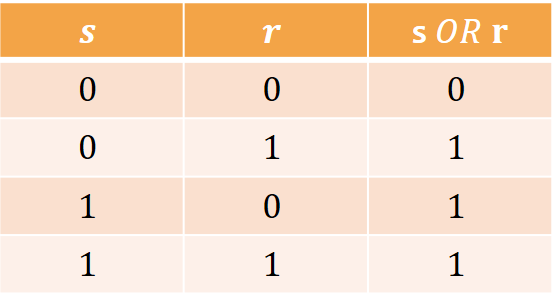
\includegraphics[width=0.4\textwidth]{Ch9/ot_or.png}
	\caption{Αρχικός πίνακας υπολογισμού OR}
	\label{fig:OT_OR}
\end{figure}

Για την αλλοίωση ο $S$ αρχικά θα επιλέξει δύο τυχαίες μεταθέσεις $v_S, v_R : \{0,1\} \rightarrow \{0,1\} $ και θα την εφαρμόσει στον πίνακα. Στη συνέχεια θα διαλέξει 4 ζεύγη από συναρτήσεις κρυπτογράφησης και αποκρυπτογράφησης:

 $$(E_0^s, D_0^s), (E_1^s, D_1^s), (E_0^r, D_0^r), (E_1^r, D_1^r)$$ 
 
 Στην συνέχεια εφαρμόζει τις συναρτήσεις κρυπτογράφησης στο αποτέλεσμα. Προκύπτει ο πίνακας \ref{fig:ot_garbled_or} ο οποίο αποστέλλεται στον $R$ μαζί με τη $v_r$.
 
 \begin{figure}
	\centering
		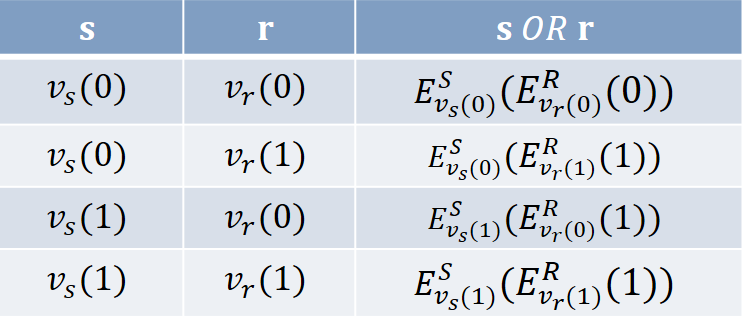
\includegraphics[width=0.6\textwidth]{Ch9/ot_garbled_or.png}
	\caption{Αλλοιωμένος πίνακας υπολογισμού OR}
	\label{fig:ot_garbled_or}
\end{figure}

Στη συνέχεια ο $S$ υπολογίζει το δικό του τμήμα του υπολογισμού δηλαδή το $v_S(s)$ και στέλνει στον $R$ το ζεύγος $(v_S(s),D_{v_S}(s)^s)$.

O $R$ τώρα υπολογίζει το $v_R(r)$. Για να αποκρυπτογραφήσει χρειάζεται την συνάρτηση $D_(v_R(r))$ την οποία όμως κατέχει ο $S$ και φυσικά πρέπει να του στείλει χωρίς όμως να αποκαλυφθεί το $v_R(r)$. Για τον σκοπό αυτό χρησιμοποιείται η Μη-Συνειδητή Μεταφορά ${OT}_1^2(S,R,D_0^R,D_1^R)$ \label{OT_ex1}. Τελικά ο $S$ μπορεί να υπολογίσει το αποτέλεσμα $D^R_{v_R(r)}(D^S_{v_S(s)}(E^S_{v_S(s)}(E^R_{v_R(r)}(x)))) $.

Δηλαδή με τη μετάθεση των γραμμών του πίνακα αλήθειας προκύπτει μία τυχαία μετάθεση του αποτελέσματος της πύλης. Κατά συνέπεια τόσο το αποτέλεσμα όσο και οι είσοδοι μπορούν να θεωρηθούν τυχαία κλειδιά. Χρειάζονται 6 ανά πύλη όπως φαίνεται στον πίνακα \ref{fig:ot_res}.

 \begin{figure}
	\centering
		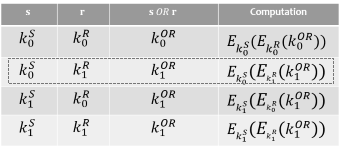
\includegraphics[width=0.6\textwidth]{Ch9/ot_res.png}
	\caption{Τελικός πίνακας υπολογισμού OR}
	\label{fig:ot_res}
\end{figure}

Για να φτιαχτεί το κύκλωμα αλλοιώνονται με τον τρόπο που περιγράψαμε παραπάνω όλες οι πύλες και συνδυάζονται τροφοδοτώντας τις εξόδους κάθε μιας στις επόμενες. Οι ενδιάμεσες έξοδοι παραμένουν κρυπτογραφημένες ενώ μόνο οι τελικές έξοδοι αποκρυπτογραφούνται από τον $R$.






